\newcommand{\duedatetime}{See Canvas for the due date}
% 16384_doc.cls lives in latex/ relative to this file; input@path lets
% \documentclass find it there without changing directory structure.
\makeatletter
\def\input@path{{latex/}}
\makeatother
\documentclass{16384_doc}

\newcommand{\assignmentname}{Assignment 3: Inverse Differential Kinematics}
\graphicspath{{latex/}}

\begin{document}
\maketitle

\tableofcontents

\section{Overview}
This assignment reinforces the following topics:
\begin{itemize}

\item Jacobians
\item Psuedoinverses

\end{itemize}

\section{Background}

\subsection{The Inverse Problem}
So far we have studied the functions that perform forward kinematics, which
means going from a manipulator's configuration space, $Q$ to its workspace, $W$:

\[
W = f(Q)
\]

\noindent In other words, we have determined the function for a robot arm that uses its
joint angles to calculate the position and orientation of its end effector (as
well as other frames on the robot).

You can probably think of a lot of cases where we want to do the inverse: given
a specified effector position (and potentially orientation), what are the joint
angles that will achieve this?  This inverse process is problematic because the
forward kinematics function, $f$, is (usually) non-linear.  That means that we
(usually) cannot just say:

\[
Q = f^{-1}(W)
\]

This means that finding the inverse function for the kinematics of an arm is
difficult (but by no means impossible---in the next assignment we will
tackle several methods to do this).

\subsection{Differential IK}
While the general problem of going from workspace positions to joint angles is
difficult, we can begin with the \emph{differential} problem -- going from
workspace velocities to configuration space velocities.
\[
\dot q = f^{-1}(\dot w)
\]

From the last assignment, you know that the function relating these two sets
of velocities is the Jacobian, $J$.  A key property of the Jacobian is that it is
linear (given the configuration $q$ of the arm).  In practical terms, this means
that if we know an arm’s joint angles and desired instantaneous end-effector
velocities, we can calculate the required joint velocities by inverting the
Jacobian:
\[
\dot q = J^{-1}(q) \dot w
\]

Because (for a given configuration) the Jacobian can be represented as a matrix, this is a much easier problem than the general IK problem we began with. It doesn't directly give us
the joint angles for a given end effector position, but it can be used to help
solve for these, as we'll see in the assignment.

\subsection{Pseudoinverse}

But wait---although inverting matrices is easy for computers, not all matrices
(and not all Jacobians) are invertible!  In order for a matrix to be invertible,
it has to be square, and have a non-zero determinant.  In terms of a robot arm
this means that it has to be:
\begin{itemize}
 \item Fully constrained (the same number of workspace and configuration space
  variables)
 \item Non-singular (the arm’s instantaneous motion can span the dimension of
  the workspace, meaning $J$ is full rank)
\end{itemize}

Fortunately, mathematicians have developed a technique called the
\emph{pseudoinverse} to help get around the problem of not having a square or
full rank matrix.  The pseudoinverse has some, but not all, of the properties of
a true matrix inverse.  The general method to compute this quantity involves
a technique called \emph{singular value decomposition}, but when the matrix is
\emph{full rank}, there are analytical formulas that can be used to find the inverse.

In this case, we basically make the matrix square by multiplying it by its
transpose.  We then invert the new matrix, and multiply the result by the
transpose of the original matrix to get the dimensions to match up. The exact
order of multiplication depends on the dimension of the matrix:

\subsubsection{Underconstrained}
To determine the joint velocities that result in a given a workspace velocity, we need to solve a system of linear equations (given a joint configuration).   If there are $n$ joint variables and $m$ workspace variables, then the Jacobian has dimensions $m \times n$.  Consider the case where $m < n$ i.e. there are more joints than the number of workspace variables. This results in a system of m equations (i.e. constraints) in n unknowns (i.e. joint velocities) where $m < n$, hence the name underconstrained.

Assuming the Jacobian is full rank, such a system always has a solution. This means we can always find joint velocities that result in a given end effector velocity. However, there is a whole family of solutions that satisfy these constraints. Therefore, one might be interested in searching the best solution in this family, measured with respect to some criterion. For the purpose of this discussion, we are interested in solutions (joint velocities) which result in the smallest effort in moving the arm. We can quantify this effort using the squared norm of the joint velocities.

Posing this as an optimization problem, we want to find $\dot q$ such that we minimize $\dot q^T \dot q$ satisfying $\dot w = J(q) \dot q$, where $\dot w$ and $J(q)$ are known.

This optimization problem is equivalent to a least-norm problem for linear systems of equations and has an exact analytical solution given by:
\[
\dot q = J^+ \dot w,
\]
% \begin{equation}
% \Qd = J^+\Wd
% \end{equation}
where $J^+$ is known as the right pseudoinverse of the Jacobian and is given by:
\[
J^+ = J^T(JJ^T)^{-1}
\]
% \begin{equation*}
% J^{+} = J^T(JJ^T)^{-1}
% \end{equation*}


\subsubsection{Overconstrained}
This case is when the number of rows the Jacobian has is greater than (or equal
to) the number of columns. In other words, there are more equations than unknowns.

In this case, the arm cannot move the end effector with the exact desired
velocity, but this solution will try to solve for the ``best'' joint velocities in
terms of the sum-squared error of end effector velocities. This is called the left puesdoinverse.
% \begin{equation*}
% J^{\#} = (J^TJ)^{-1}J^T
% \end{equation*}
\[
J^\# = (J^TJ)^{-1}J^T
\]

As a side note, the pseudoinverse in this overconstrained case is really useful
even outside of kinematics, and is used to quickly and reliably do things like
solve for best-fit lines to data.

\subsubsection{Perfectly Constrained}
Note that in the case of a square full rank matrix, the psuedoinverse will
result in $J^{-1}$.

\subsection{Course Logistics}

In this class you would be using the following websites regularly:
\begin{itemize}
    \item \href{https://canvas.cmu.edu/courses/56566}{Canvas}: The main course web page. This links to everything relevant to the class (including the next two links).
    \item \href{https://piazza.com/class/mt8vtez94dv38b}{Piazza}: This is the best way to ask course staff questions, and see course announcements.
    \item \href{https://www.gradescope.com/courses/1369131}{Gradescope}: This is where you will be turning in your homework. You should have already been added to the course. If you haven't, please contact the course staff via email or Piazza post.
\end{itemize}

You can write your \verb!writeup.pdf! in \href{https://www.overleaf.com/}{Overleaf}: upload the assignment zip as a new project, and use \verb!assignment3.tex! as your template (it pulls in \verb!16384_doc.cls! and the figures from the \verb!latex/! folder automatically).

\writtenSection

\section{Written Questions}
% For all of the following questions, please fully compute all answers and show
% your work for full credit, unless otherwise specified. Submit your answers in a
% PDF entitled \verb!writeup.pdf! in your handin directory.  All answers must be
% typed, but diagrams may be hand-drawn and scanned in.  However, they must be
% tidy and fully legible! Consider drawing them in a black or blue pen.  All units
% are in radians and meters, where appropriate.

\begin{questions}

    \titledquestion{R Robot}
    Consider the following robot
    \begin{center}
    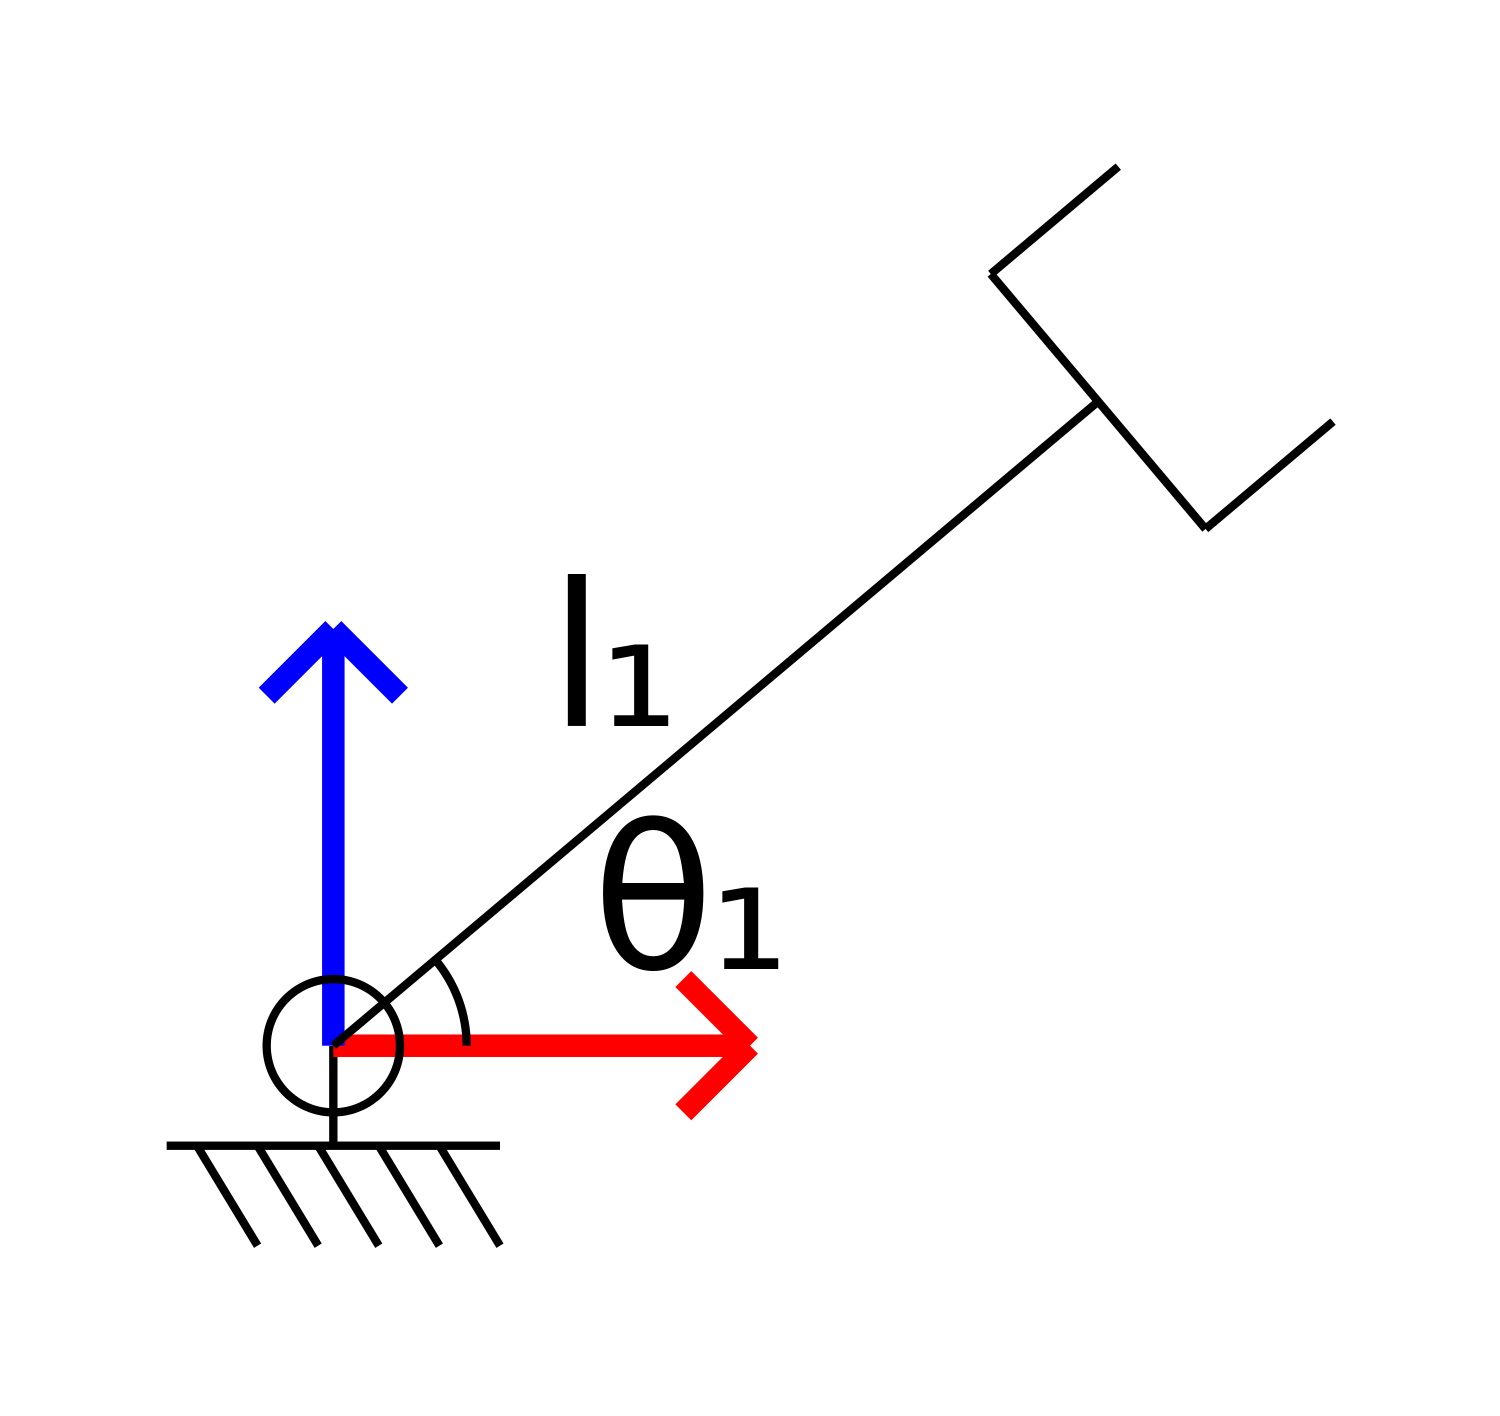
\includegraphics[scale=0.07]{generated_figures/R_nonsingular.png}
    \end{center}

        Assume \th[1] = \piover{4}.
    \begin{enumerate} [label=\alph*.]
        \item \text{[1 point]} What is the dimension of the end-effector Jacobian? Consider
        end-effector positions $\begin{bmatrix} x\\ y \end{bmatrix}$ in $\mathbb{R}^2$.
        \begin{tcolorbox}[height=3cm]
            % TODO: ENTER YOUR ANSWER HERE
        \end{tcolorbox}
        
        \item \text{[1 point]} Is this system underconstrained, overconstrained, or neither?
        Why?
        \begin{tcolorbox}[height=3cm]
            % TODO: ENTER YOUR ANSWER HERE
        \end{tcolorbox}

        
        \item \text{[2 points]} Draw the velocity vector for the end effector caused by joint 1
        moving with unit velocity. The direction of these vectors should be
        correct, but do not worry about the magnitude. You can complete this
        problem by inspection or by using properties of the Jacobian.

        \begin{tcolorbox}[height=8cm]
            % TODO: ENTER YOUR ANSWER HERE
        \end{tcolorbox}

        \item \text{[2 points]} What is the dimension of the space spanned by this vector?
        \begin{tcolorbox}[height=3cm]
            % TODO: ENTER YOUR ANSWER HERE
        \end{tcolorbox}
        
        \item \text{[1 point]} What is the rank of $J$ for this configuration?
        \begin{tcolorbox}[height=3cm]
            % TODO: ENTER YOUR ANSWER HERE
        \end{tcolorbox}
        
        \item \text{[1 point]} When identifying the inverse differential kinematics for this
        problem, would you use the inverse, the left psuedoinverse, or the right
        psuedoinverse?
        \begin{tcolorbox}[height=3cm]
            % TODO: ENTER YOUR ANSWER HERE
        \end{tcolorbox}
        
        \item \text{[3 points]} What are the benefits of a left pseudoinverse versus a right
        pseudoinverse?
        \begin{tcolorbox}[height=3cm]
            % TODO: ENTER YOUR ANSWER HERE
        \end{tcolorbox}
        
    \end{enumerate}

    \titledquestion{RR Robot}
    Consider the following robot
    \begin{center}
    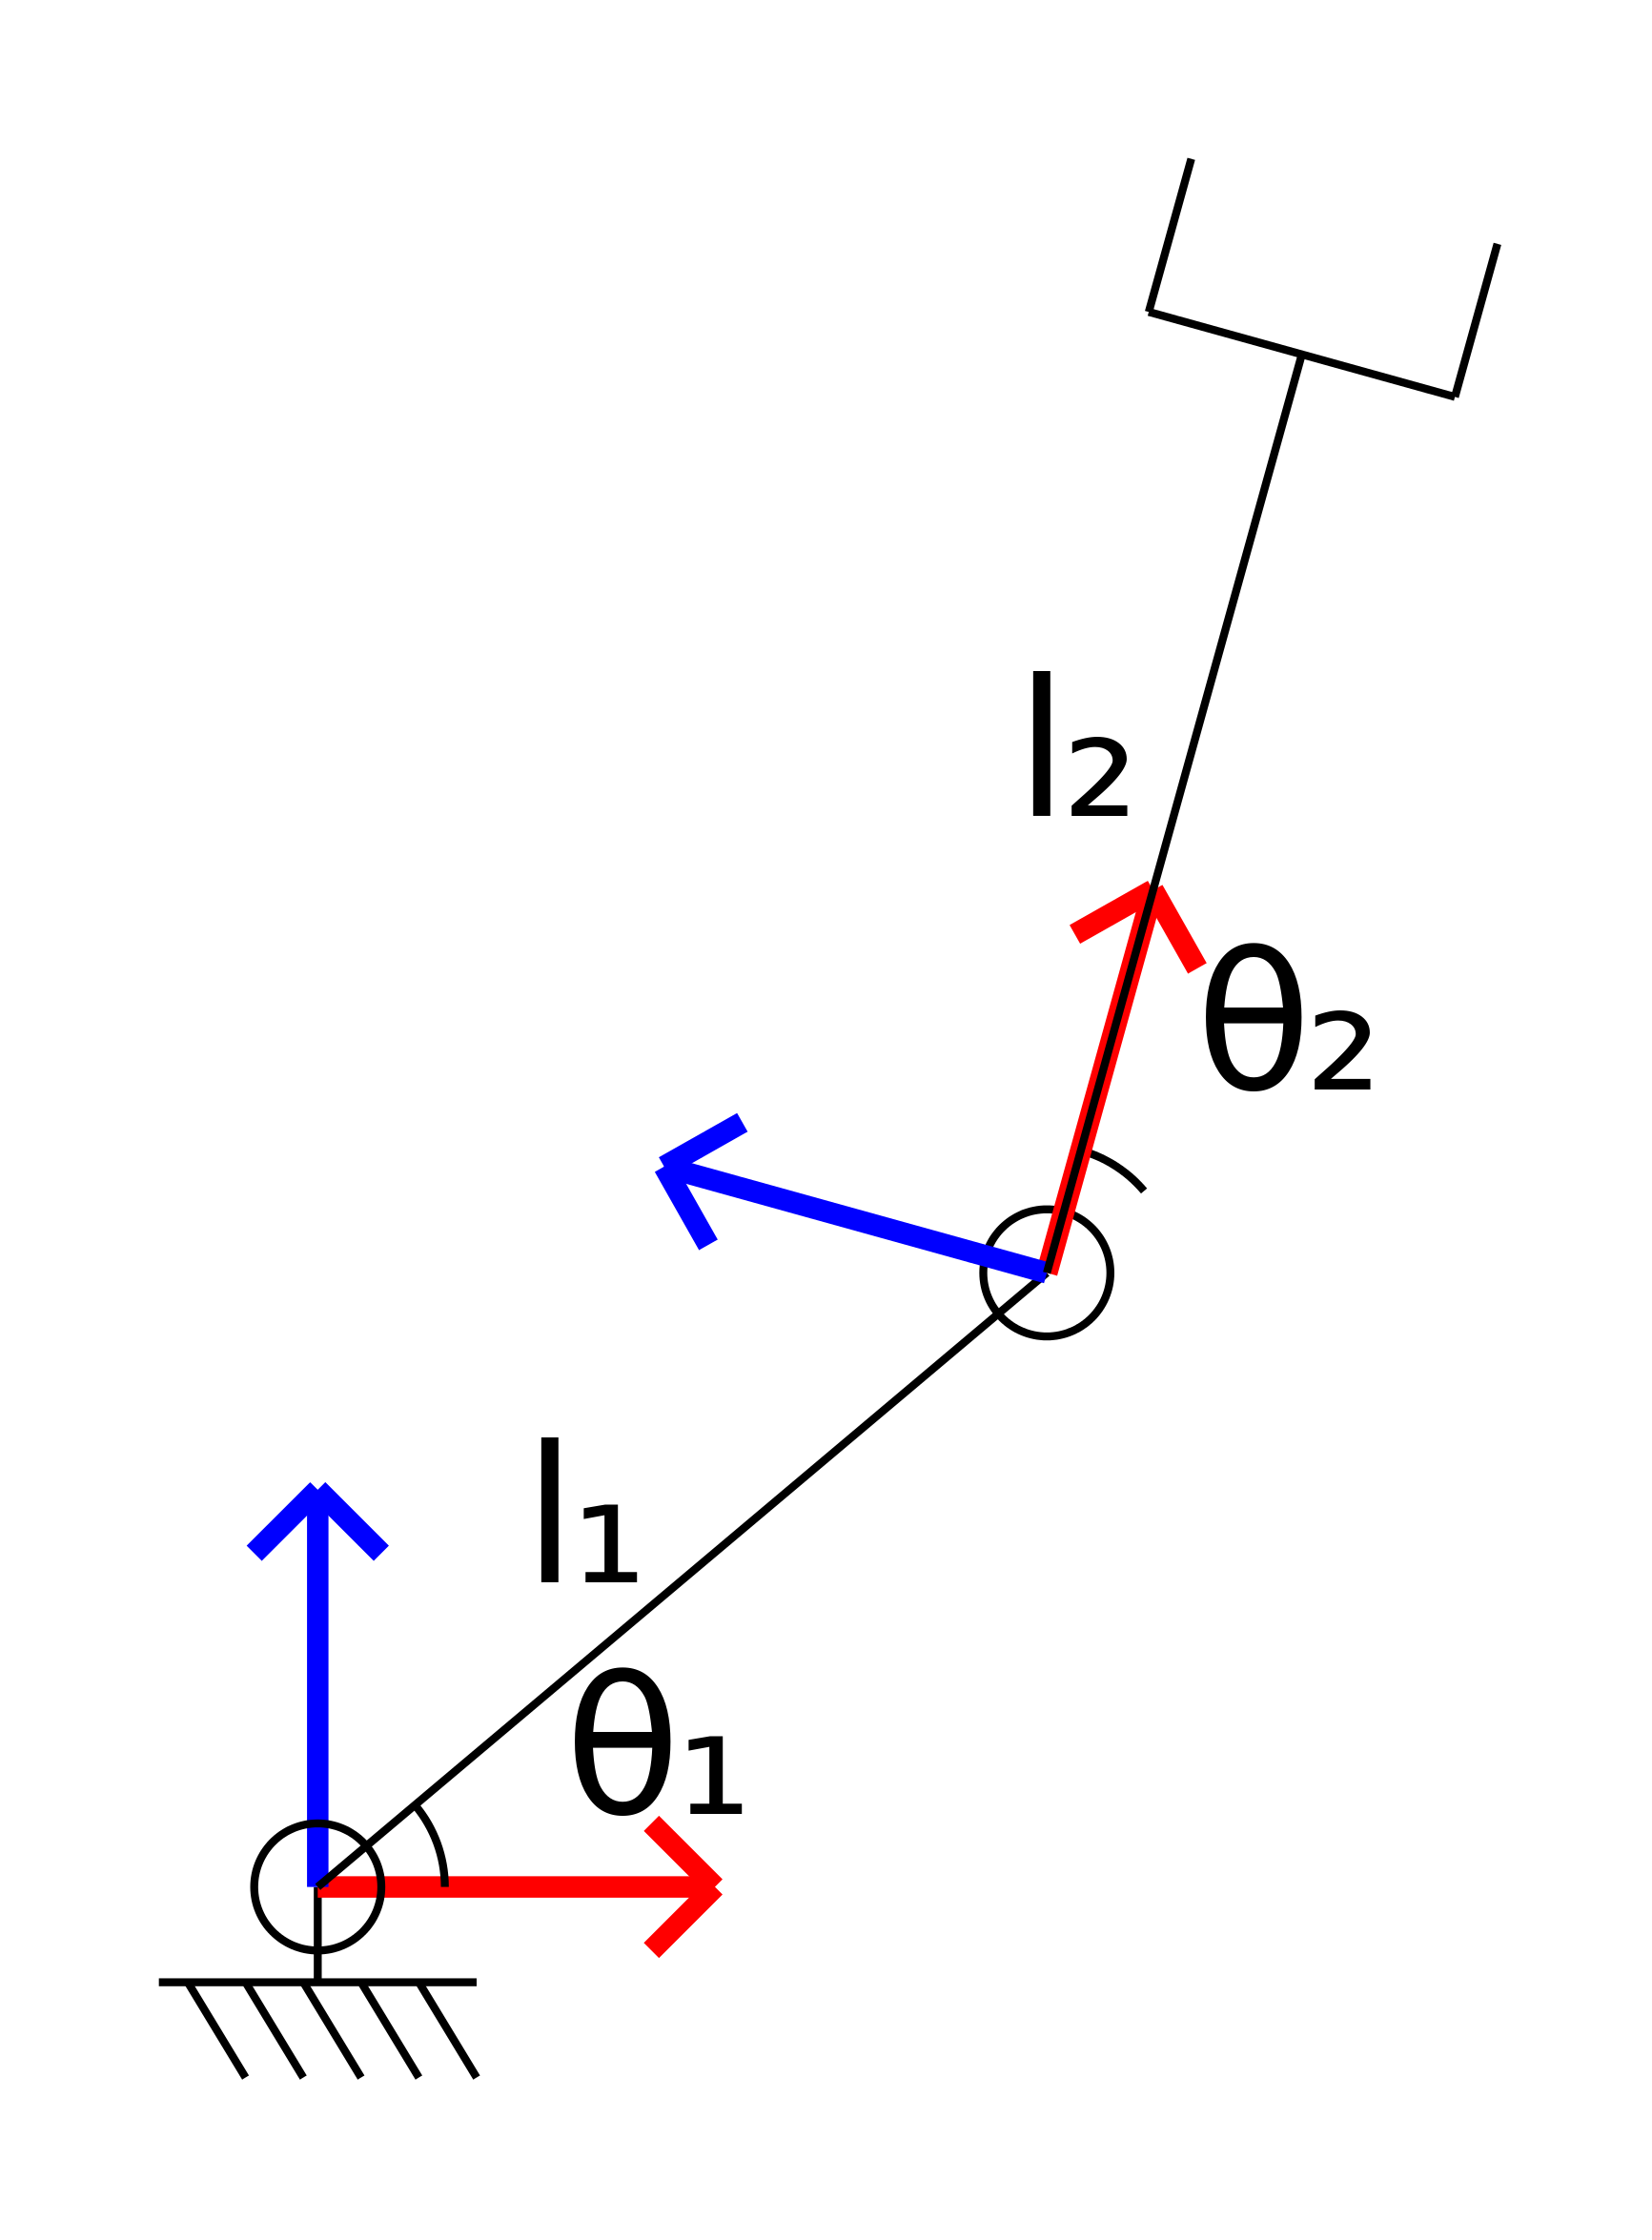
\includegraphics[scale=0.07]{generated_figures/RR_nonsingular.png}
    \end{center}
        Assume $\begin{bmatrix}
            \theta_1 \\
            \theta_2
        \end{bmatrix} = \begin{bmatrix}
            \frac\pi4 \\
            \frac\pi4
        \end{bmatrix}$.
        % \smcolvec{\th[1]\\\th[2]} =
        % \smcolvec{\piover{4}\\\piover{4}}.
    \begin{enumerate} [label=\alph*.]
        \item \text{[1 point]} What is the dimension of the end-effector Jacobian? Consider
        end effector positions $\begin{bmatrix} x \\ y \end{bmatrix} \in \mathbb{R}^2$.%\smcolvec{x\\y} in $\RR^2$.
        \begin{tcolorbox}[height=3cm]
            % TODO: ENTER YOUR ANSWER HERE
        \end{tcolorbox}
        
        \item \text{[1 point]} Is this system underconstrained, overconstrained, or neither?
        Why?
        \begin{tcolorbox}[height=3cm]
            % TODO: ENTER YOUR ANSWER HERE
        \end{tcolorbox}
        
        \item \text{[4 points]} On separate plots, draw the velocity vector for the end effector
        caused by:
        \begin{enumerate} [label=(\roman*)]
          \item Joint 1 moving with unit velocity (joints 2 has zero velocity).
          \item Joint 2 moving with unit velocity (joints 1 has zero velocity).
        \end{enumerate}
        The direction of these vectors should be correct, and the relative
        magnitudes should be approximately correct, but do not worry about
        exact magnitudes.  You can complete this problem by inspection or by
        using properties of the Jacobian.
        \begin{tcolorbox}[height=8cm]
            % TODO: ENTER YOUR ANSWER HERE
        \end{tcolorbox}

        \item \text{[2 points]} What is the dimension of the space spanned by these vectors?
        Are the 1st and 2nd vectors linearly independent?
        \begin{tcolorbox}[height=3cm]
            % TODO: ENTER YOUR ANSWER HERE
        \end{tcolorbox}
        
        \item \text{[1 point]} What is the rank of $J$ for this configuration?
        \begin{tcolorbox}[height=3cm]
            % TODO: ENTER YOUR ANSWER HERE
        \end{tcolorbox}
        
        \item \text{[1 point]} When identifying the inverse differential kinematics for this
        problem, would you use the inverse, the left psuedoinverse, or the right
        psuedoinverse?
        \begin{tcolorbox}[height=3cm]
            % TODO: ENTER YOUR ANSWER HERE
        \end{tcolorbox}
        
    \end{enumerate}

    \titledquestion{RRR Robot}
    Consider the following robot
    \begin{center}
    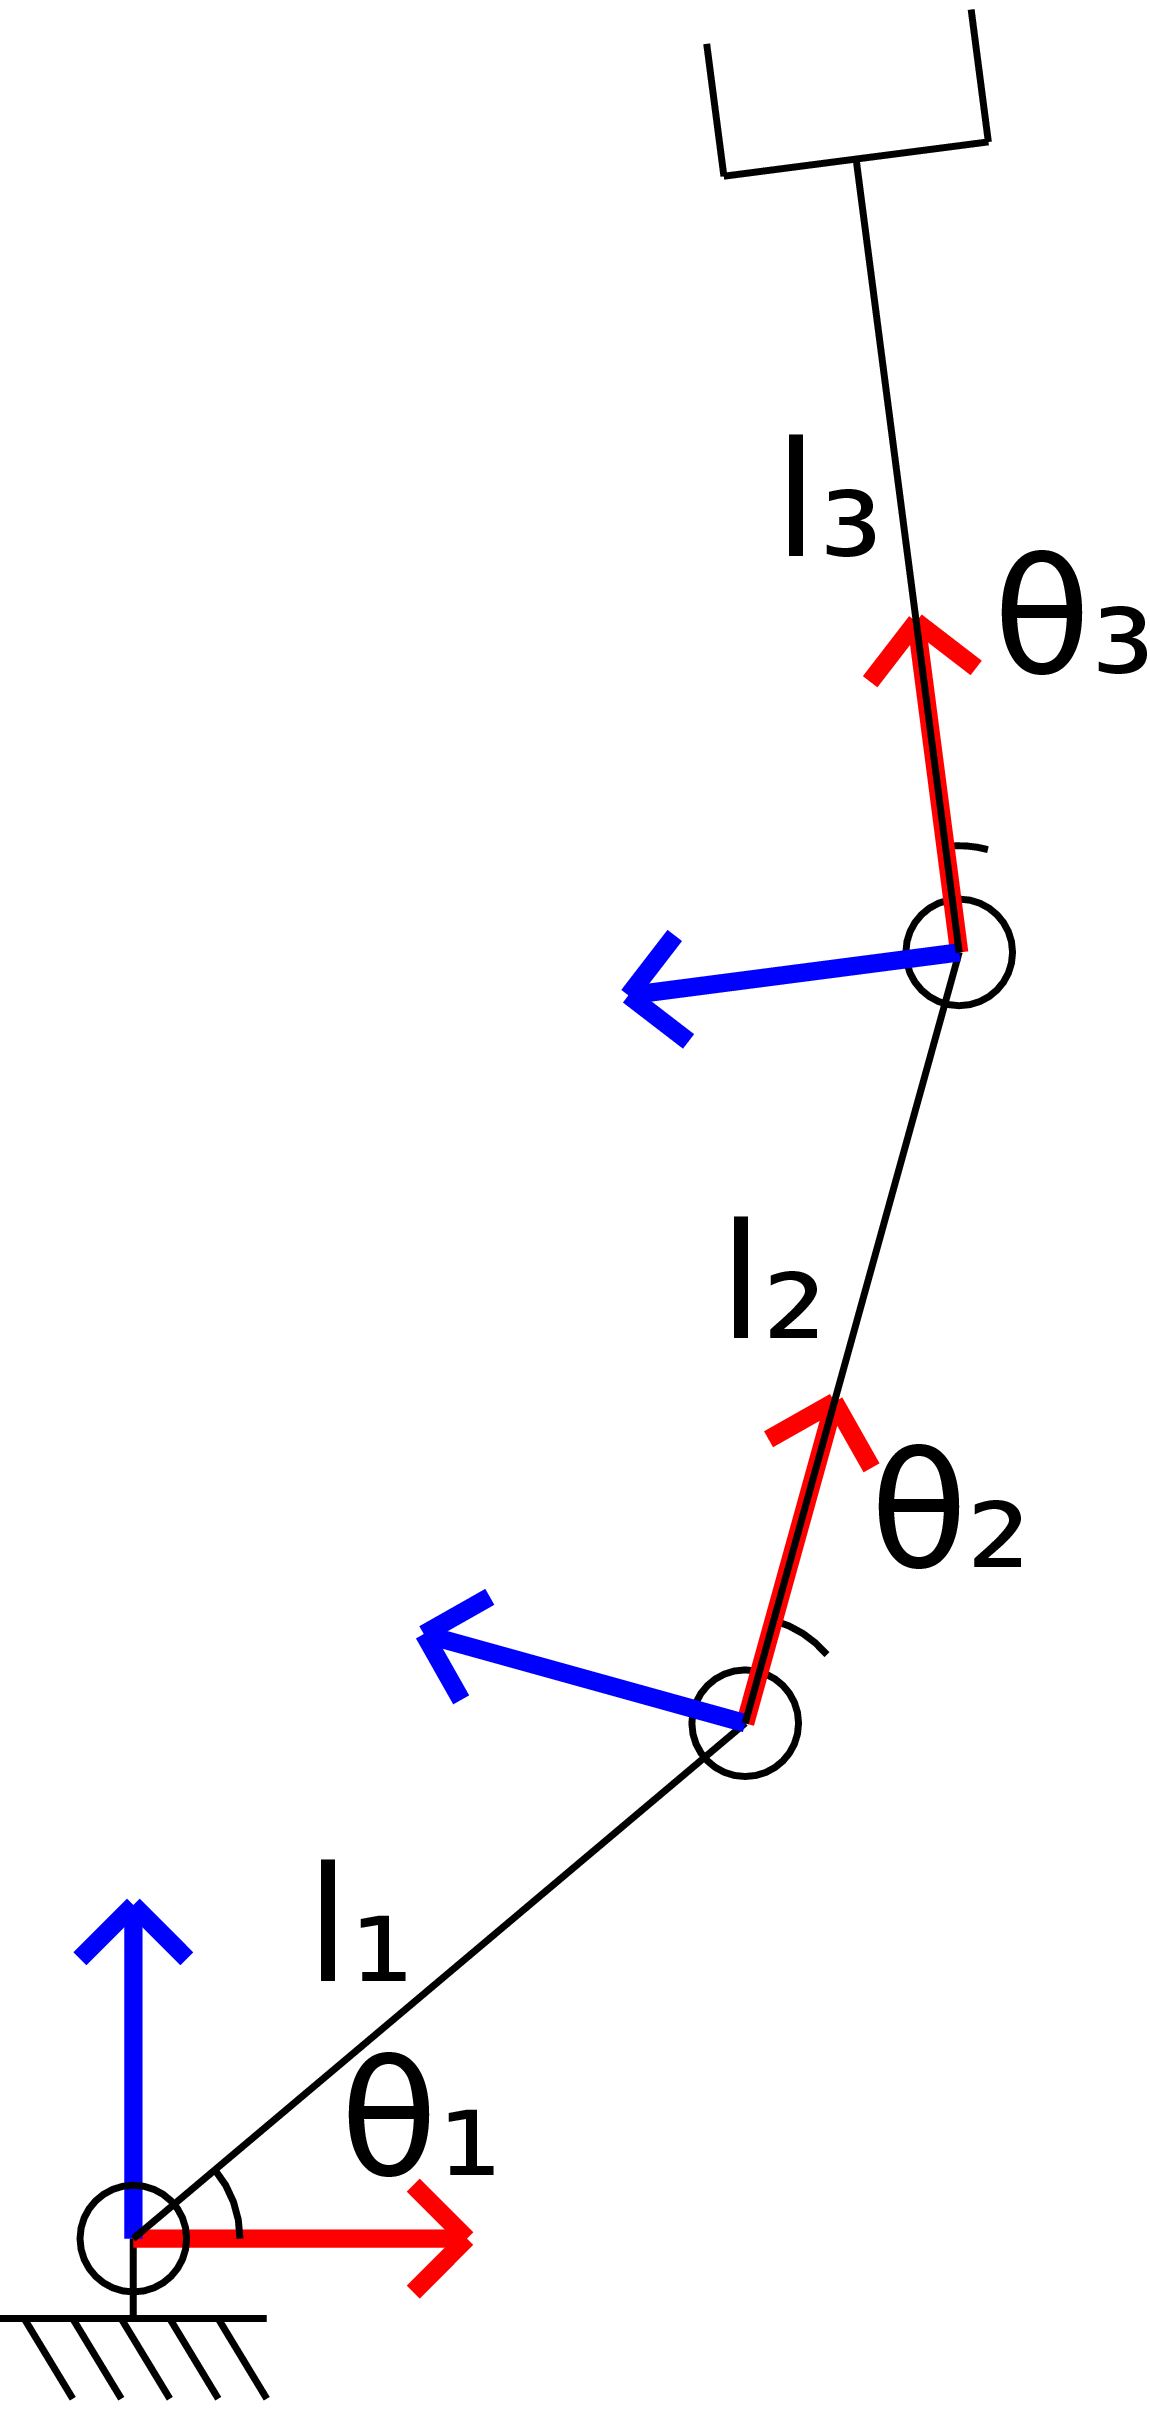
\includegraphics[scale=0.07]{generated_figures/RRR_nonsingular.png}
    \end{center}

    Assume $\begin{bmatrix}
        \theta_1 \\ \theta_2 \\ \theta_2
    \end{bmatrix} = \begin{bmatrix}
        \frac\pi3 \\ \frac\pi3 \\ \frac\pi3
    \end{bmatrix}$.
    % \smcolvec{\th[1]\\\th[2]\\\th[3]} =
    % \smcolvec{\piover{2}\\\piover{3}\\\piover{3}}.
    
     \begin{enumerate} [label=\alph*.]
        \item \text{[1 point]} What is the dimension of the end-effector Jacobian? Consider
        end effector positions $\begin{bmatrix}
            x \\ y
        \end{bmatrix} \in \mathbb{R}^2$. %\smcolvec{x\\y} in $\RR^2$.
        \begin{tcolorbox}[height=3cm]
            % TODO: ENTER YOUR ANSWER HERE
        \end{tcolorbox}
        
        \item \text{[1 point]} Is this system underconstrained, overconstrained, or neither?
        Why?
        \begin{tcolorbox}[height=3cm]
            % TODO: ENTER YOUR ANSWER HERE
        \end{tcolorbox}
        
        \item \text{[6 points]} On separate plots, draw the velocity vector for the end effector
        caused by
        \begin{enumerate} [label=(\roman*)]
          \item Joint 1 moving with unit velocity (joints 2 and 3 have zero velocity).
          \item Joint 2 moving with unit velocity (joints 1 and 3 have zero velocity).
          \item Joint 3 moving with unit velocity (joints 1 and 2 have zero velocity).
        \end{enumerate}
        The direction of these vectors should be correct, and the relative
        magnitudes should be approximately correct, but do not worry about
        exact magnitudes.  You can complete this problem by inspection or by
        using properties of the Jacobian.
        \begin{tcolorbox}[height=6.5cm]
            % TODO: ENTER YOUR ANSWER HERE
        \end{tcolorbox}

        \item \text{[2 points]} What is the dimension of the space spanned by these vectors?
        Are the 1st and 2nd vectors linearly independent? The 1st and 3rd?  The
        2nd and 3rd? All three?
        \begin{tcolorbox}[height=3cm]
            % TODO: ENTER YOUR ANSWER HERE
        \end{tcolorbox}
        
        \item \text{[1 point]} What is the rank of $J$ for this configuration?
        \begin{tcolorbox}[height=3cm]
            % TODO: ENTER YOUR ANSWER HERE
        \end{tcolorbox}
        
        \item \text{[1 point]} When identifying the inverse differential kinematics for this
        problem, would you use the inverse, the left psuedoinverse, or the right
        psuedoinverse?
        \begin{tcolorbox}[height=3cm]
            % TODO: ENTER YOUR ANSWER HERE
        \end{tcolorbox}
        
    \end{enumerate}

    \titledquestion{RRR Robot, revisited with rotation}

    Consider the following robot
    \begin{center}
    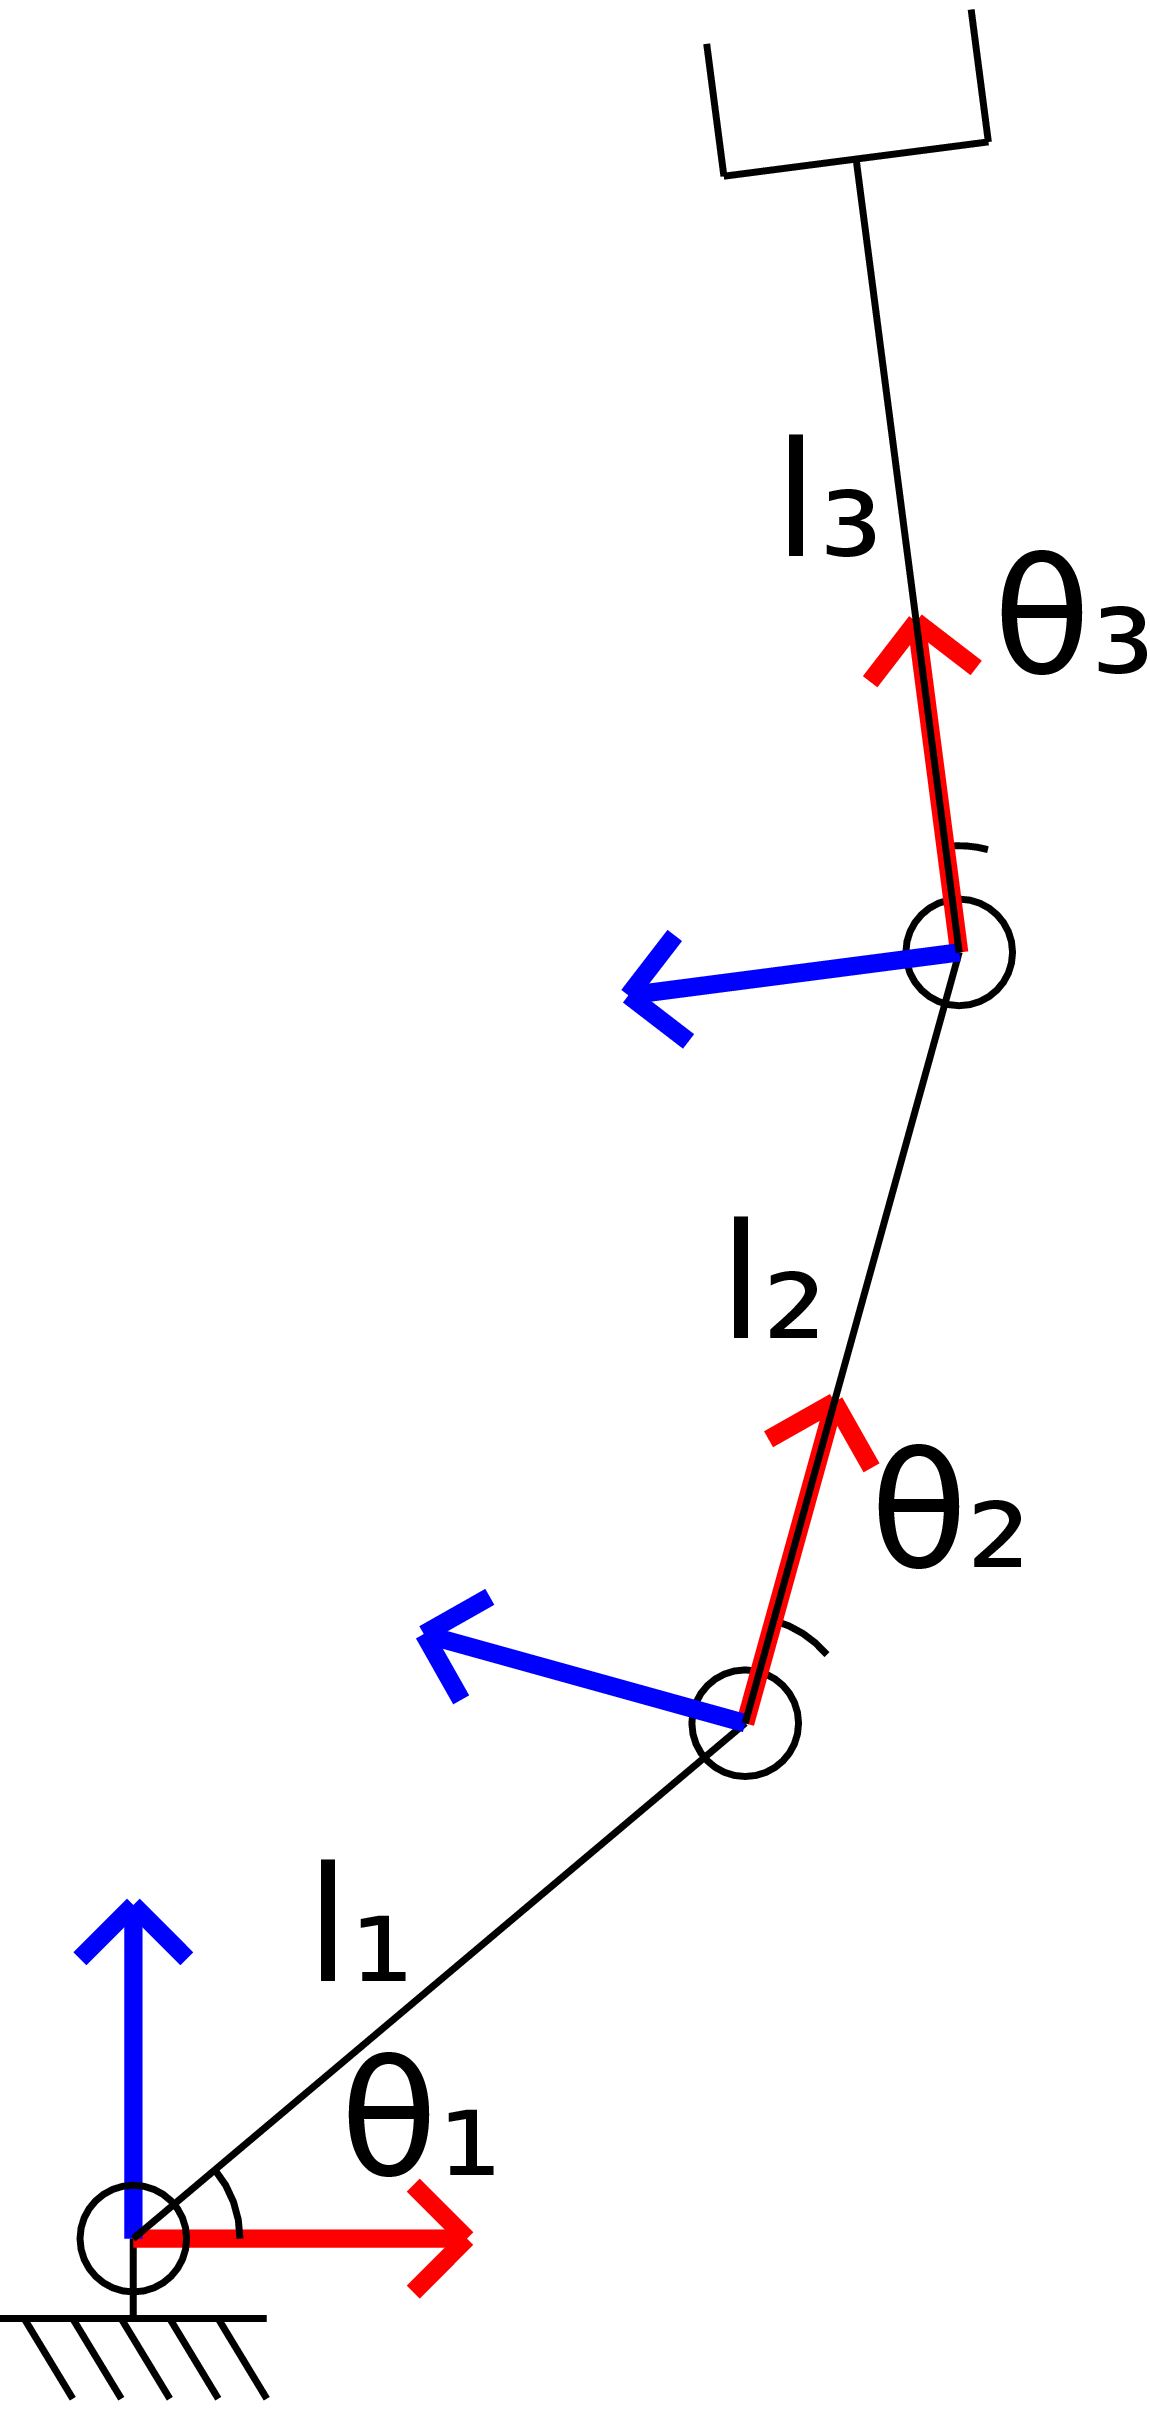
\includegraphics[scale=0.07]{generated_figures/RRR_nonsingular.png}
    \end{center}
    \begin{enumerate} [label=\alph*.]
        \item \text{[1 point]} What is the dimension of the end-effector Jacobian, now considering
        $\begin{bmatrix}
            x \\ y \\ \theta
        \end{bmatrix}$
        %\smcolvec{x\\y\\\th}
        end-effector positions in $SE(2)$.
        \begin{tcolorbox}[height=3cm]
            % TODO: ENTER YOUR ANSWER HERE
        \end{tcolorbox}
        
        \item \text{[1 point]} Is this system underconstrained, overconstrained, or neither?
        Why?
        \begin{tcolorbox}[height=3cm]
            % TODO: ENTER YOUR ANSWER HERE
        \end{tcolorbox}
        
        \item \text{[1 point]} Write out the end-effector Jacobian.
        \begin{tcolorbox}[height=3cm]
            % TODO: ENTER YOUR ANSWER HERE
        \end{tcolorbox}
        
        \item \text{[3 points]} Assume $\theta_1 = 0.6$, $\theta_2 = 0.6$, and $\theta_3 = 0.4$ (all
        values in radians). Write out the end-effector velocity $\begin{bmatrix} \dot x \\ \dot y \\ \dot z \end{bmatrix}$
        %\smcolvec{\xd\\\yd\\\thd} 
        for each of:
        \begin{enumerate} [label=(\roman*)]
          \item Joint 1 moving with unit velocity (joints 2 and 3 have zero velocity).
          \item Joint 2 moving with unit velocity (joints 1 and 3 have zero velocity).
          \item Joint 3 moving with unit velocity (joints 1 and 2 have zero velocity).
        \end{enumerate}
        \begin{tcolorbox}[height=3cm]
            % TODO: ENTER YOUR ANSWER HERE
        \end{tcolorbox}
        
        \item \text{[2 points]} What is the dimension of the space spanned by these vectors? Are
        the 1st and 2nd vectors linearly independent? The 1st and 3rd?  The 2nd
        and 3rd? All three?
        \begin{tcolorbox}[height=3cm]
            % TODO: ENTER YOUR ANSWER HERE
        \end{tcolorbox}
        
        \item \text{[1 point]} What is the rank of $J$ for this configuration?
        \begin{tcolorbox}[height=3cm]
            % TODO: ENTER YOUR ANSWER HERE
        \end{tcolorbox}
        
        \item \text{[2 points]} When identifying the inverse differential kinematics for this
        problem, would you use the inverse, the left psuedoinverse, or the right
        psuedoinverse?
        \begin{tcolorbox}[height=3cm]
            % TODO: ENTER YOUR ANSWER HERE
        \end{tcolorbox}
    \end{enumerate}

    \titledquestion{RRR Singular Configuration}

    Consider the following robot
    \begin{center}
    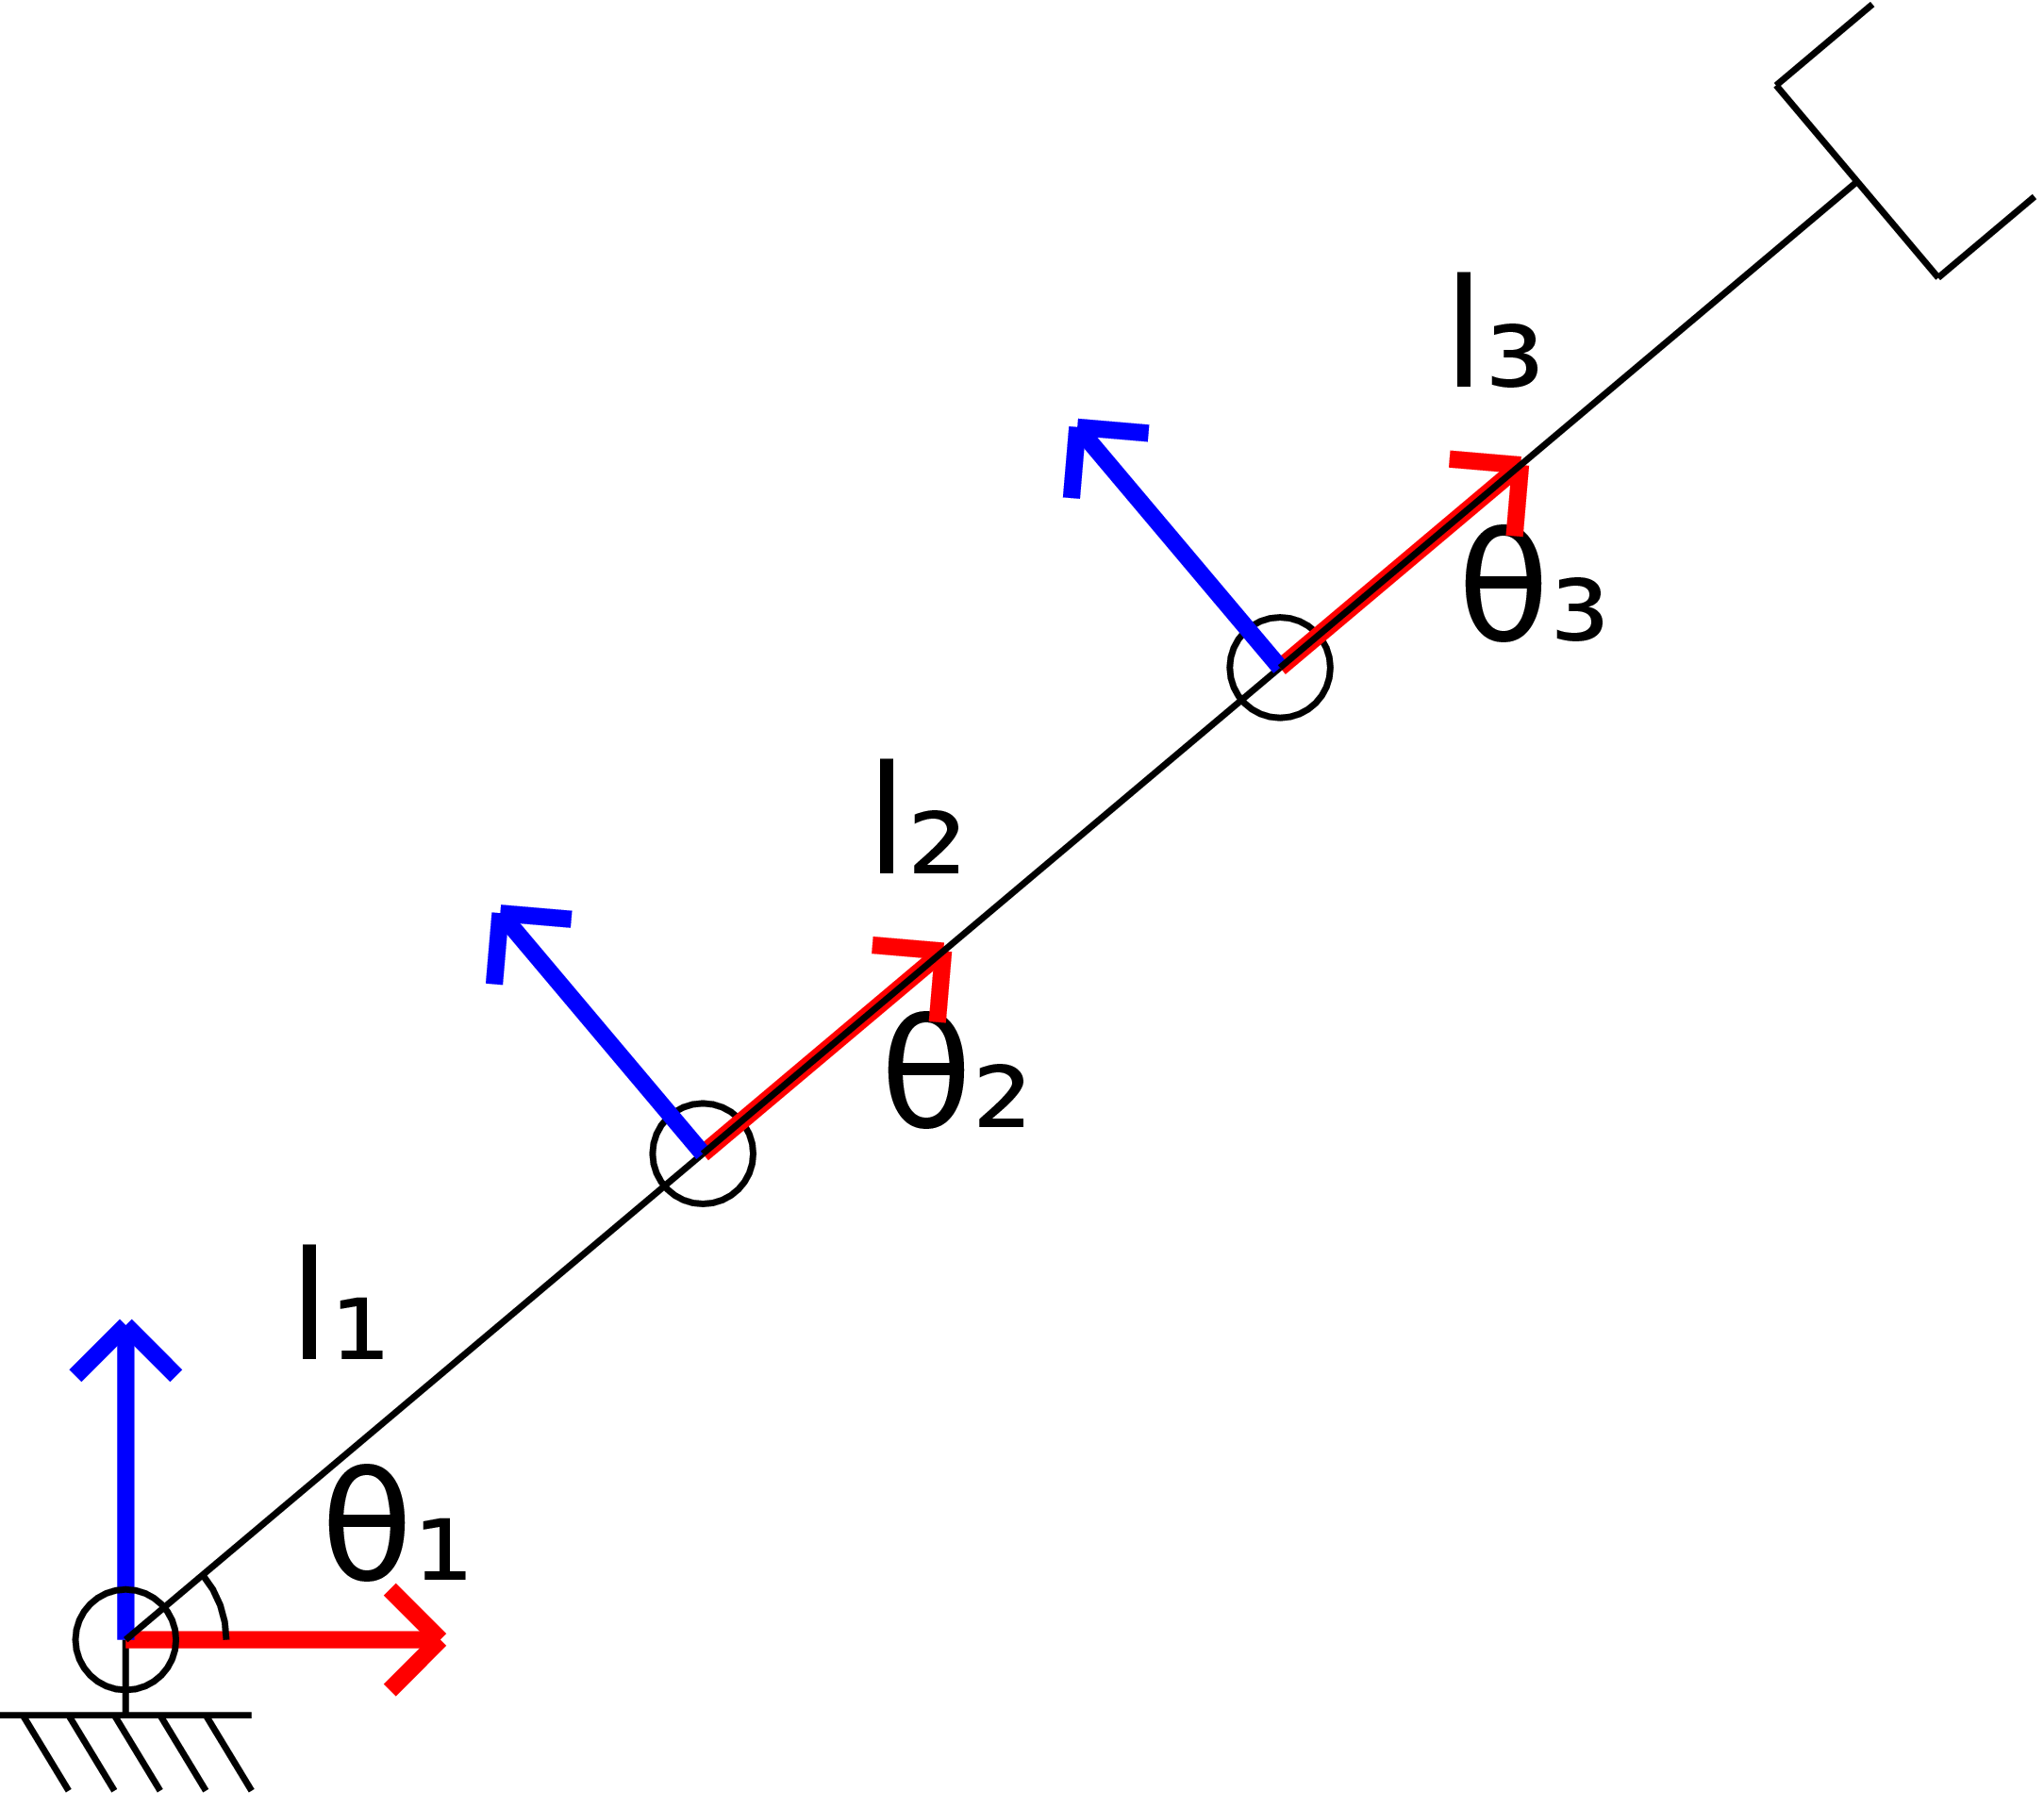
\includegraphics[scale=0.07]{generated_figures/RRR_singular.png}
    \end{center}
    \begin{enumerate} [label=\alph*.]
        \item \text{[1 point]} What is the dimension and rank of the end-effector Jacobian?
        Consider end effector positions $\begin{bmatrix} x \\ y \end{bmatrix} \in \mathbb{R}^2$.
        %\smcolvec{x\\y} in $\RR^2$.
        Do the dimension
        and rank differ? why?
        \begin{tcolorbox}[height=3cm]
            % TODO: ENTER YOUR ANSWER HERE
        \end{tcolorbox}
        
        \item \text{[6 points]} On separate plots, draw the velocity vector for the end effector
        caused by
        \begin{enumerate} [label=(\roman*)]
          \item Joint 1 moving with unit velocity (joints 2 and 3 have zero velocity).
          \item Joint 2 moving with unit velocity (joints 1 and 3 have zero velocity).
          \item Joint 3 moving with unit velocity (joints 1 and 2 have zero velocity).
        \end{enumerate}
        The direction of these vectors should be correct, and the relative
        magnitudes should be approximately correct, but do not worry about
        exact magnitudes.  You can complete this problem by inspection or by
        using properties of the Jacobian.
        \begin{tcolorbox}[height=6cm]
            % TODO: ENTER YOUR ANSWER HERE
        \end{tcolorbox}

        \item \text{[2 points]} What is the dimension of the space spanned by these vectors? Are
        the 1st and 2nd vectors linearly independent? The 1st and 3rd?  The 2nd
        and 3rd? All three?
        \begin{tcolorbox}[height=3cm]
            % TODO: ENTER YOUR ANSWER HERE
        \end{tcolorbox}
        
        \item \text{[1 point]} What is the rank of $J$ for this configuration?
        \begin{tcolorbox}[height=3cm]
            % TODO: ENTER YOUR ANSWER HERE
        \end{tcolorbox}
        
    \end{enumerate}

    \titledquestion{Local Inverse Kinematics}

    Consider a general arm with revolute joints. Assume you already have the
    kinematic map to the end effector, $f$, and the Jacobian of the end
    effector, $J$.

    The robot arm begins with joint angles $\Theta_0$, resulting in an
    end-effector position of $\mathbf{p}_0 = f(\Theta_0)$.  The end effector
    needs to pick up an object at point $\mathbf{p}_1$.

    Note: this is a conceptual problem: do not consider joint limits, and
    assume that all relevant positions are within the workspace of the robot.
    Furthermore, all answers are in terms of the given variables and known
    constants.
    
    \begin{enumerate} [label=\alph*.]
        \item \text{[2 points]} What are the initial joint angle velocities $\dot{\Theta}_0$ that
      start to move the end effector directly towards $\mathbf{p}_1$?
      \begin{tcolorbox}[height=3cm]
            % TODO: ENTER YOUR ANSWER HERE
        \end{tcolorbox}
        
        \item \text{[3 points]} Assume the end effector has moved at $\dot{\Theta}_0$ for a small
      amount of time $dt$.  What joint angles velocities $\dot{\Theta}_{dt}$
      will move the end effector from this new starting point directly towards
      $\mathbf{p}_1$?
      \begin{tcolorbox}[height=3cm]
            % TODO: ENTER YOUR ANSWER HERE
        \end{tcolorbox}
        
        \item \text{[2 points]} Describe (in a couple of sentences) how you would command the
      robot to move from $\mathbf{p}_0$ to $\mathbf{p}_1$ in approximately 1
      second.
      \begin{tcolorbox}[height=3cm]
            % TODO: ENTER YOUR ANSWER HERE
        \end{tcolorbox}
        
    \end{enumerate}

    Note that this process describes how differential IK can be used to solve
    IK \emph{numerically}, given a nearby starting point.  We will explore this
    concept in more depth in the next assignment.

\end{questions}


\section{Code Questions}
  
Ensure Python and the
NumPy and Matplotlib libraries are correctly installed.

For Python installation, visit:
\begin{center}
    \href{https://www.python.org/downloads/}{https://www.python.org/downloads/}
\end{center}
For NumPy and Matplotlib, install via pip:
\begin{verbatim}
    pip install numpy matplotlib
\end{verbatim}

After setting up, download the \verb!code! folder from the \href{https://github.com/CMU-16384-2026-Fall/Assignment3}{GitHub repository} and navigate to that location. Whenever you work on the assignment, run your scripts from inside this directory.

\begin{questions}
    \titledquestion{\text{[50 points]} General Robot Class}
    Open directory \verb!code!.
    For this exercise, we will walk you through the creation of a general Python
    class representing a fixed-base kinematic chain. You will implement
    forward kinematics for any RR arm.
    First, open the file \verb!Robot.py!, and study this file. This is a basic Python
    class. The idea here is that you can pass parameters to the \emph{constructor} of
    the robot class, and the returned object then has methods that can be
    called, and can operate on the values you passed in. For example, the
    following code:
    \begin{verbatim}
    robot = Robot(np.array([[0.55], [0.4]]),\
    np.array([[1], [1]]), np.array([[1], [1]]), 0)

    
    frames = robot.fk(np.array([[0], [np.pi/2]]))
    \end{verbatim}
    can be used to find the forward kinematics of a robot with link lengths of
    0.55 and 0.4 for $\theta = \begin{bmatrix} 0 \\ \frac\pi2 \end{bmatrix}$
    \begin{center}
    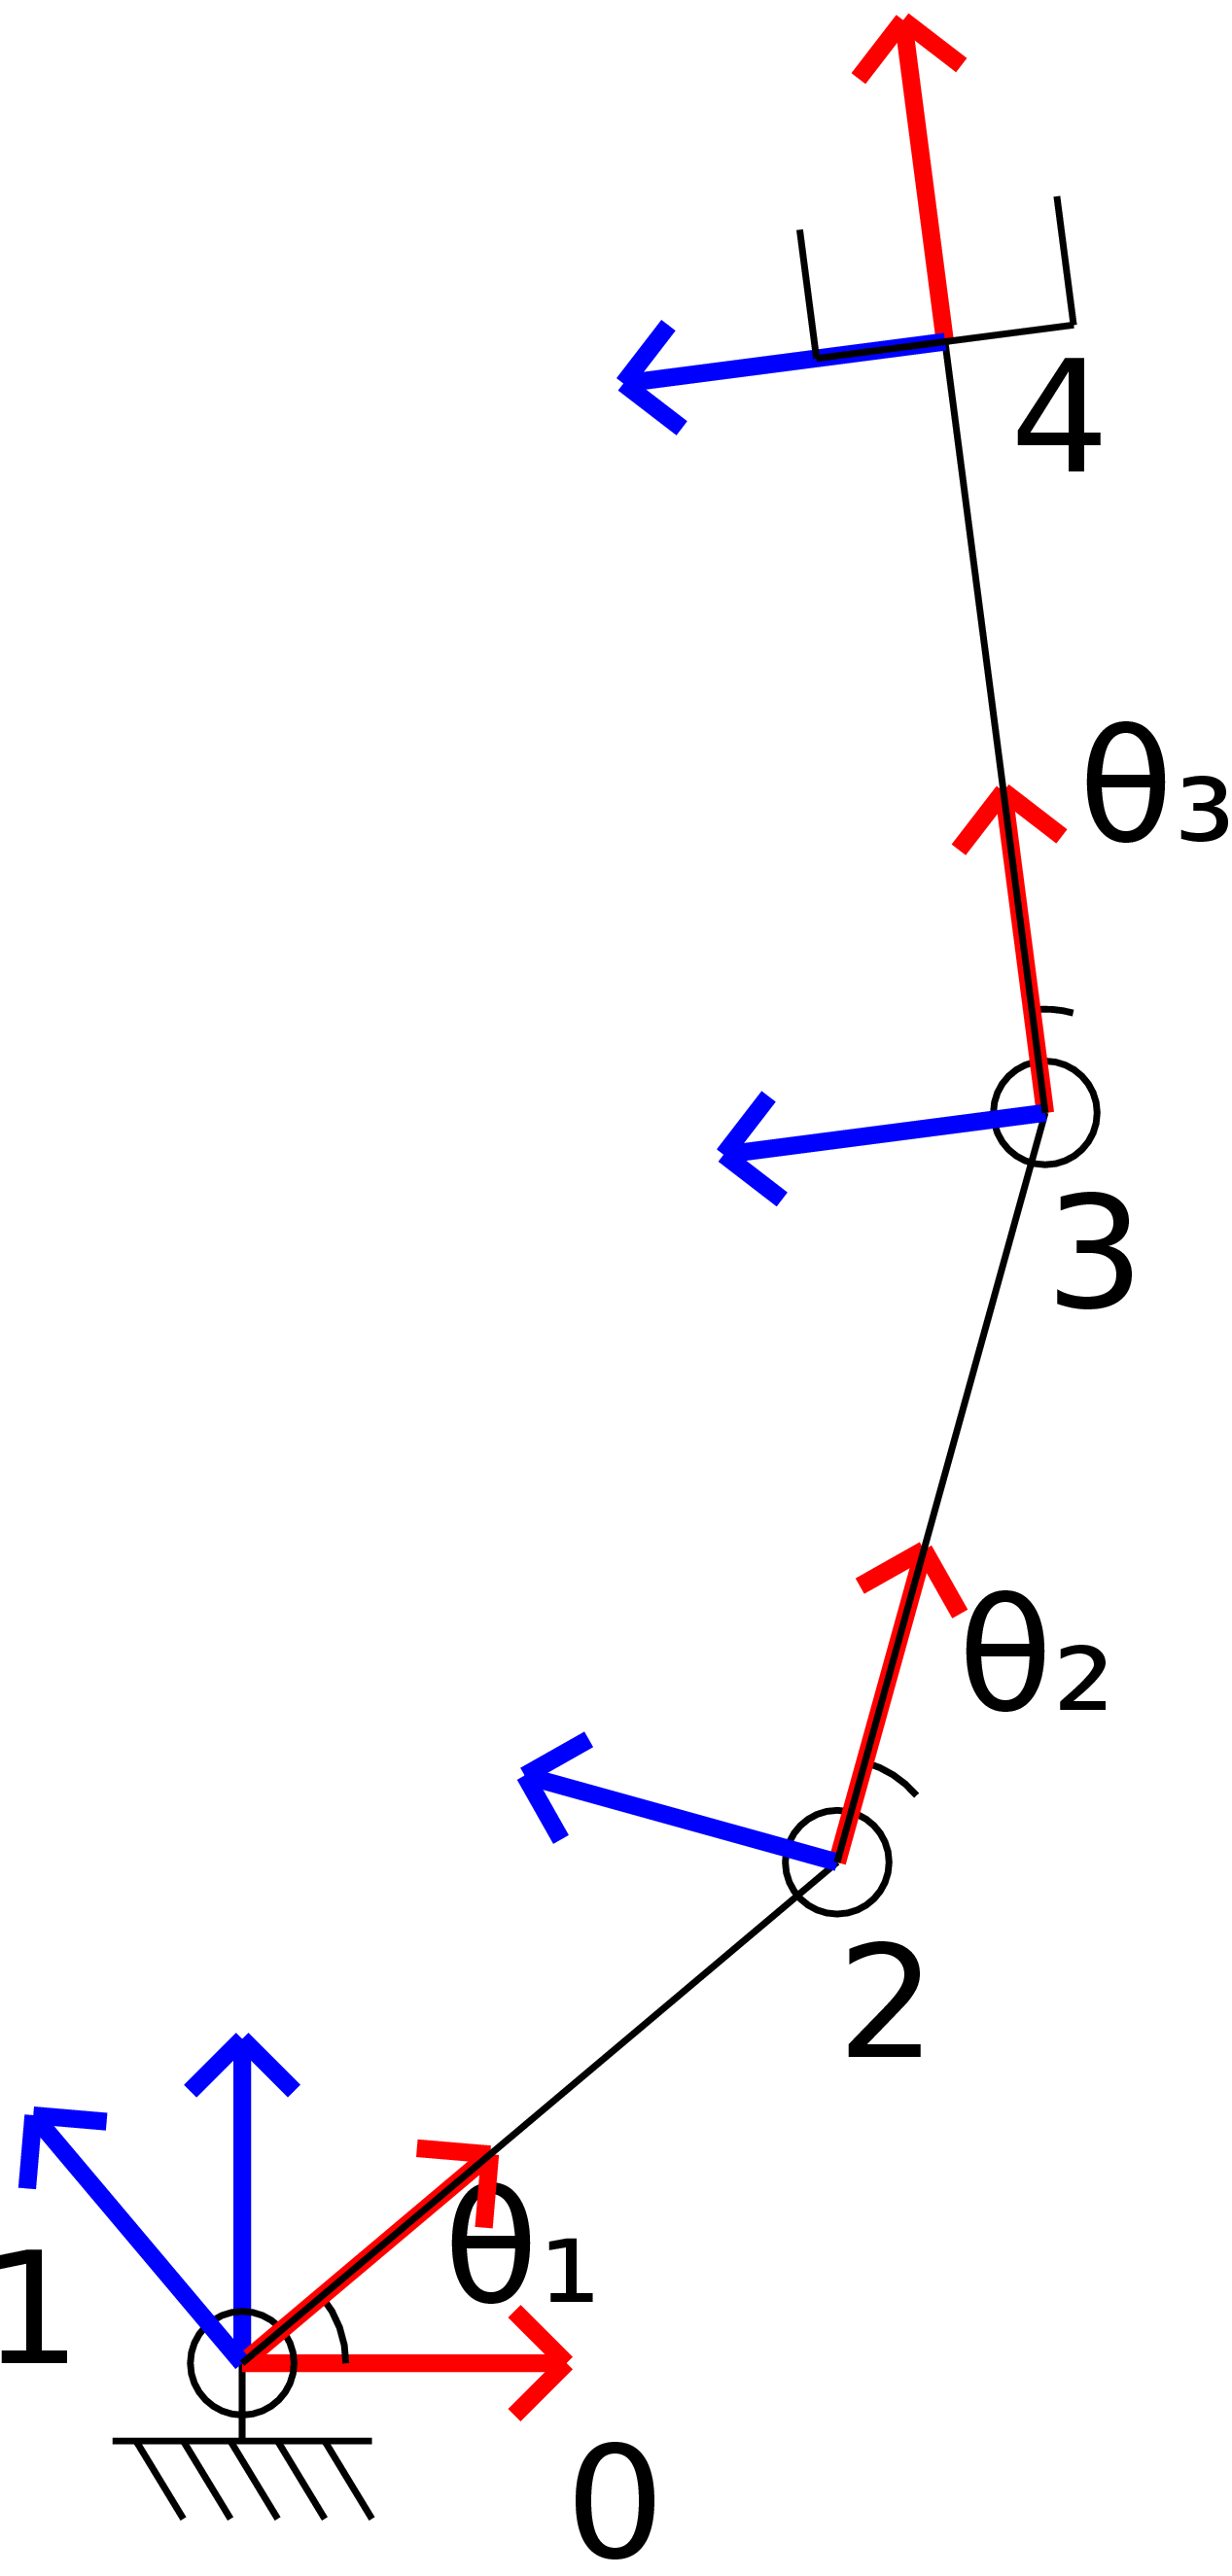
\includegraphics[scale=0.07]{generated_figures/RRR_alltheframes.png}
    \end{center}
    \paragraph{Forward Kinematics} Your job is to write forward kinematics that
    can work for any number of revolute joints in a chain. You will fill in
    the \verb!forward_kinematics! method in the \verb!Robot! class. This computes
    $H_i^0$ for each frame ($i > 0$) in the figure above, including the end
    effector frame.
    The code describes the conventions used for the resulting variable.
    One suggestion that should help is to break this problem into three
    components:
    \begin{itemize}
      \item First consider frame 1.
      \item Use a for loop to iterate from frame 2 to $n-1$; use 
      $H_{i-1}^0$ to help compute frame $H_i^0$.
      \item Compute the end effector frame, using $H_{n-1}^0$ to help.
    \end{itemize}
    \paragraph{Verification and Submission} To verify your results:
    \begin{enumerate}
      \item Run the \verb!sample_path! function. This will generate a plot and save
            two CSV files: \verb!calculated_path.csv! and \verb!ground_truth_path.csv!.
            This is for your own reference, to check whether your output matches
            the sample test case.
      \item Run the local self-check before submitting: from the
            \verb!local_autograder! directory, run
            \begin{verbatim}
python local_autograder.py
            \end{verbatim}
            This runs your \verb!Robot.fk! over 25 published test arms (chain
            lengths 2 through 6) and prints PASS/FAIL for each. A FAIL message
            tells you what to look for:
            \begin{itemize}
              \item \verb!<n>/<total> poses off by > 1 cm! --- \verb!fk! runs
                    but returns the wrong position; check your homogeneous
                    transforms.
              \item \verb!raised <ExceptionType>: <message>! --- \verb!fk!
                    crashed; the message says where.
              \item \verb!end-effector path has the wrong shape or is not finite!
                    --- your output isn't the expected $(N, 2)$ array, or it
                    contains NaN/inf.
            \end{itemize}
      \item The autograder on Gradescope will check your implementation against
            the same 25 arms and joint angles, but perturbs each one a little
            and checks against the reference solution instead of a file. If the
            local check above passes, you should pass on Gradescope too.
      \item To submit your work:
        \begin{itemize}
          \item Run the \verb!create_submission.py! script provided in the \verb!code! directory.
                This will zip up all necessary files in the \verb!code! folder.
          \item Submit the resulting zip file to Gradescope.
        \end{itemize}
    \end{enumerate}
    Save your sample path plot as a PNG and include it in your writeup. Also include
    an explanation of your forward kinematics implementation and any challenges you
    encountered.
\end{questions}

\section{Hands-on Lab}

% STAFF TODO (not for students): clean up the student workstations before the
% lab opens --- there are grippers lying around on several of them.

So far the arms in this assignment have been drawings.  In this section you will
put your own kinematics on a real one: a seven-joint UFACTORY xArm7, driven as
the planar RR arm you have been working with all along.  You will implement its
forward kinematics and its Jacobian, check them against the simulator from your
own machine, and then --- in lab --- push the real arm by hand through a path of
your choosing and watch it replay that path while your kinematics draw it live.

% TODO: fill in the lab room and workstation names, the access hours, and
% whether students sign up for a slot or walk in.
The robots live in the \emph{Robotics Engineering Lab}.  Please be mindful of
others and share the robots fairly: check Piazza for signups.

\subsection{The xArm7 as a Planar RR Arm}

The xArm7 has seven revolute joints; the arm in the written questions has two,
in a plane.  The two become the same mechanism once four of the seven joints are
held still.  Holding
\[
    \th[2] = \piover{2}, \quad
    \th[3] = \piover{2}, \quad
    \th[5] = -\piover{2}, \quad
    \th[6] = \piover{2}
\]
leaves joints 1 and 4 turning about axes that are both parallel to the world
$z$-axis, so the end effector moves in a horizontal plane and the arm is an RR
arm lying on its side.  (Joint 7 is left free as well, but its axis is that same
vertical one and it only spins the tool about itself, so it does not move the
point you are tracing.)  Joints 1 and 4 are the \emph{free} joints, and their
angles --- after a fixed offset, which \verb!robot_info.py! handles for you ---
are the $\th[1]$ and $\th[2]$ of your RR arm.

The two links are not round numbers, because they come from where the xArm7's
joints actually are: $\l[1] = 0.2977$ m from the shoulder to the elbow and
$\l[2] = 0.4256$ m from the elbow to the wrist.  Read them from
\verb!robot_info()['link_lengths']! rather than typing them in --- the starter
code already does this for you.

\subsection{Setting Up}

The lab code needs the course robot library, \verb!xarm7_lib!.  If you installed
it earlier in the semester, update it, since the version this assignment needs is
newer:
\begin{verbatim}
    git clone https://github.com/CMU-16384-2026-Fall/16384-robot-lib
    cd 16384-robot-lib
    git pull                        # if you already had it cloned
    conda activate 16384            # if not already activated
    conda env update -f environment.yml
    conda activate 16384
\end{verbatim}

\noindent Then get this assignment's lab code, which is the \verb!lab! folder of
the same \href{https://github.com/CMU-16384-2026-Fall/Assignment3}{GitHub
repository} you downloaded \verb!code! from:
\begin{verbatim}
    cd Assignment3/lab
\end{verbatim}

\noindent Run every command in this section from inside that \verb!lab! folder.
Work in a Git repository that you can push from and pull onto the lab machine:
you will write your code on your own machine, and the fastest way to get it onto
the robot's computer is \verb!git pull!.

The same scripts drive either the real arm or a MuJoCo simulation, and they
choose between them by looking at the \verb!ROBOT_IP! environment variable: set,
and they talk to the arm at that address; unset, and you get the simulation.  So
everything below except the recording itself can be developed and debugged at
home, with no robot.

\begin{questions}

    \titledquestion{\text{[50 points]} Tracing a Path on the xArm7}

    This question is graded by hand, from one video you record in lab.  Read the
    deliverable at the end before you go, so you know what the video has to show.

    \begin{center}
        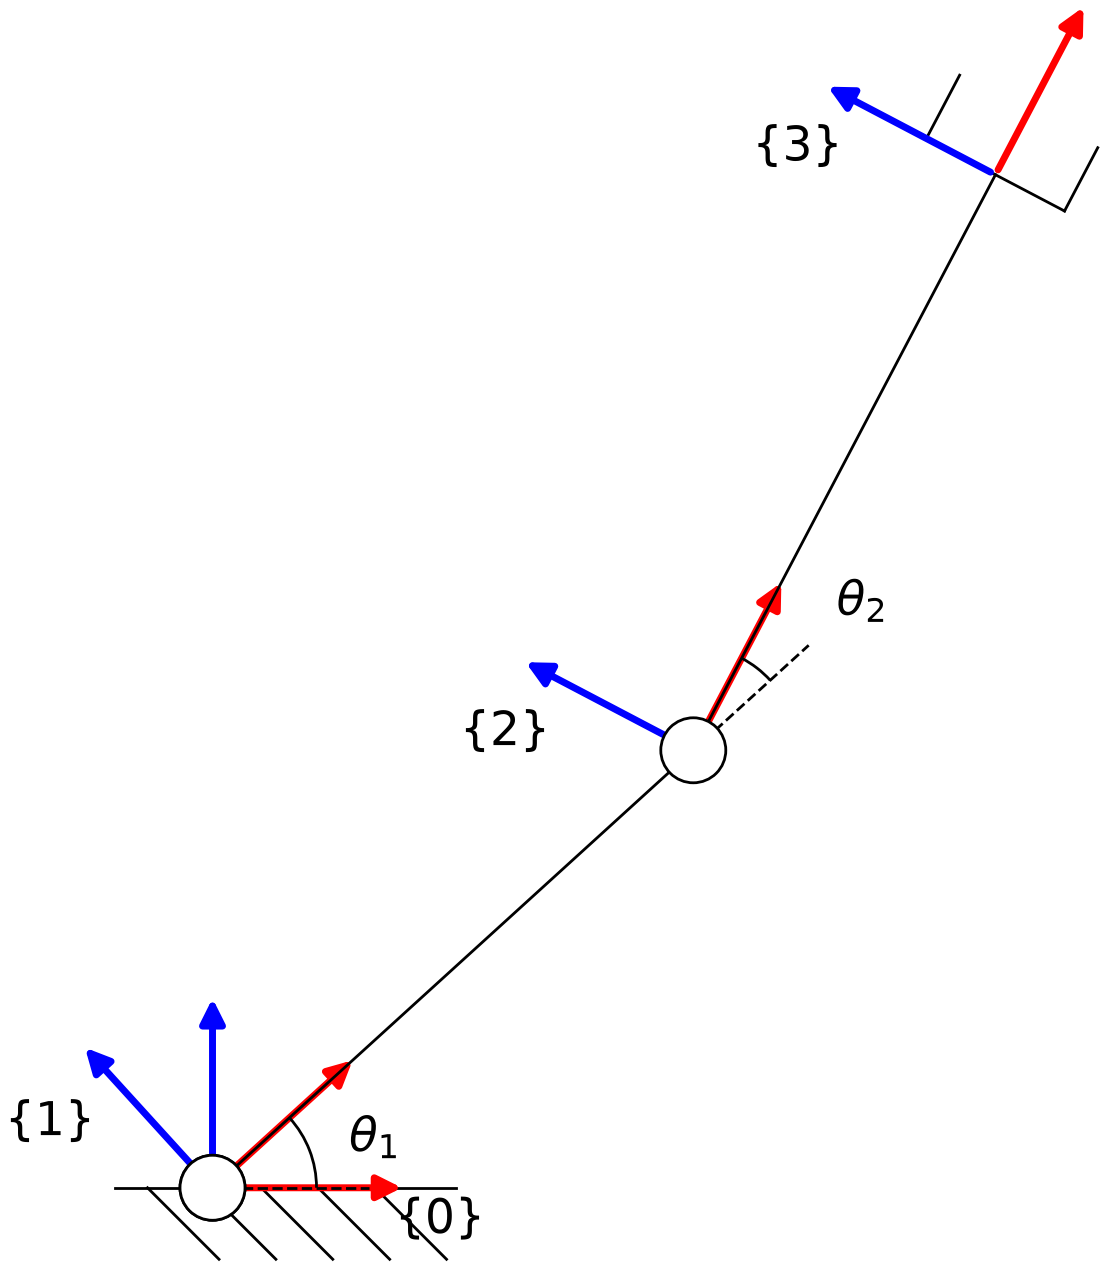
\includegraphics[width=0.3\textwidth]{generated_figures/RR_lab.png}
    \end{center}

    \paragraph{To-Do 1: Forward Kinematics} Open \verb!fk.py! and fill in
    \verb!forward_kinematics_RR!, which returns two $3\times3$ planar homogeneous
    transforms for frames $\{2\}$ and $\{3\}$. The frames are labeled in the figure above.

    \paragraph{To-Do 2: The Jacobian} Fill in \verb!jacobian_RR!, the $2\times2$
    end-effector \emph{position} Jacobian $\J$ at $(\th[1], \th[2])$: column $i$
    is how fast the end effector moves, and in what direction, when joint $i$
    turns at unit speed.  It is what turns joint velocities into the end
    effector's velocity,
    \[
        \colvec{\xd \\ \yd} = \J(\th[1], \th[2]) \colvec{\thd[1] \\ \thd[2]},
    \]
    and the plot below draws exactly that product as an arrow off the end
    effector, so a correct Jacobian is something you can see.

    \paragraph{Checking Your Work in Simulation} The \verb!lab! folder ships a
    sample recording, \verb!square.csv!, so you can test both functions before you
    ever touch a robot.  On your own machine, run:
    \begin{verbatim}
        python replay.py square.csv
    \end{verbatim}
    Two windows open: the simulated xArm7 in a browser tab (its address is also
    printed as \verb!Meshcat: <url>! when the script starts), and a top-down plot
    of the arm drawn entirely by \emph{your} code.  The plot is drawn as if you
    were standing in front of the robot, looking down: the base is at the top,
    the robot's $+x$ axis points down the screen towards you, and its $+y$ axis
    to your right.  In it you should see a plot like the following screenshot:

    \begin{center}
        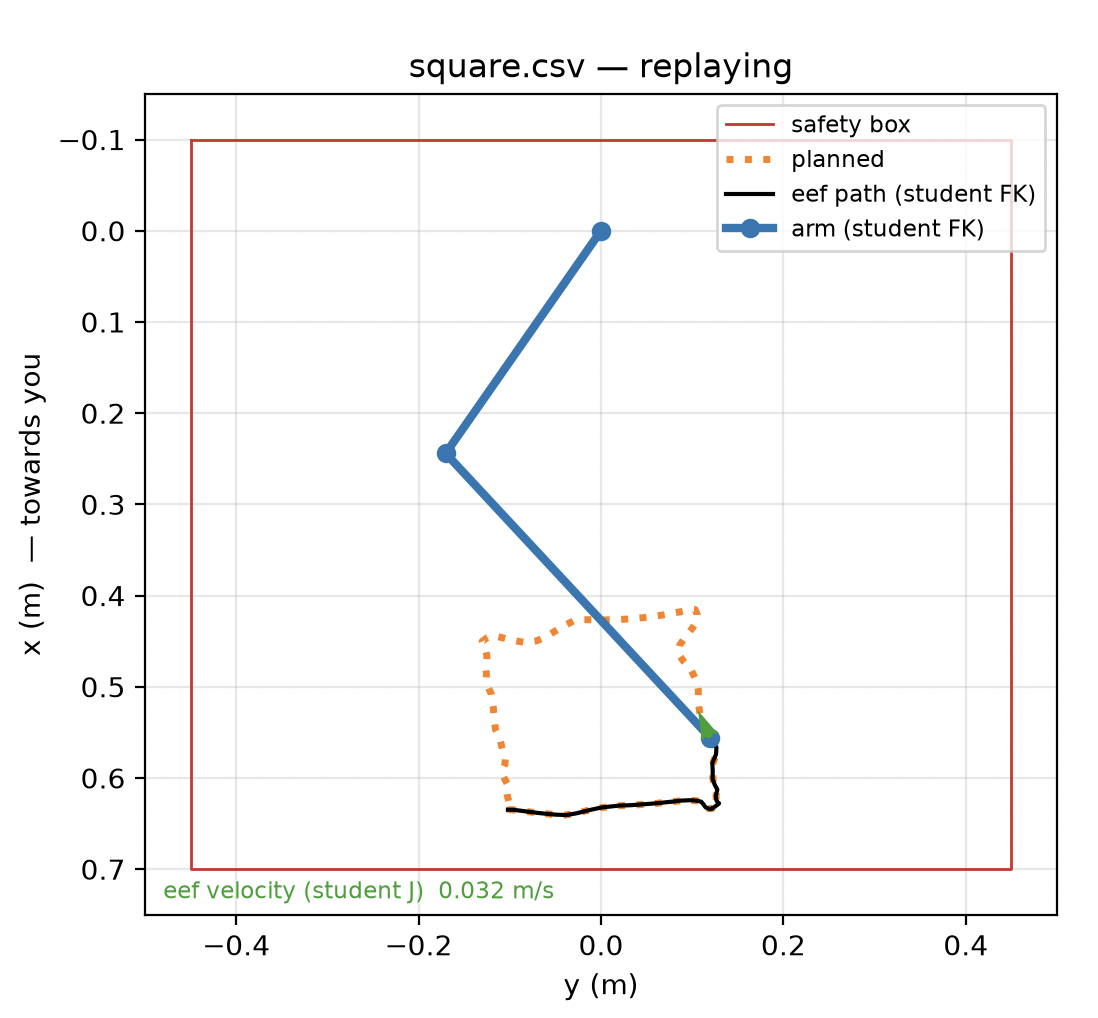
\includegraphics[width=0.5\textwidth]{generated_figures/replay_screenshot.png}
    \end{center}

    Your code in \verb|fk.py| will determine the blue arm, the black \& orange paths, and the green arrow. Those should match the above screenshot at some point in time. Note that the estimated velocity (green arrow) is noisy, so it will fluctuate during the replay.

    If something is off, the symptom tells you which To-Do to look at:
    \begin{itemize}
      \item The drawn arm does not match the simulated arm --- \verb!forward_kinematics_RR!.
            Note that only the translation column of each transform is used to draw
            the arm, so check the rotation blocks too; they can be wrong while the
            picture still looks reasonable.
      \item The path is right but the arrow points the wrong way, or has
            the wrong length --- \verb!jacobian_RR!.
    \end{itemize}
    Sort all of this out before your lab session; the arm is a slow place to
    debug a sign error.

    \begin{tcolorbox}[colback=red!5, colframe=red!60!black,
        title={Safety: Read this before you touch the robot}]
    \begin{itemize}
      \item \textbf{Powering on.} Ask a TA during their office hours to walk you through powering up and
            enabling your station the first time.  Do not power-cycle the
            controller yourself if the arm is in an unexpected state; ask.
      \item \textbf{The e-stop.} Know where the emergency stop button is
            \emph{before} you start, and keep it within reach.  Press it for
            anything you did not expect --- an unexpected motion, a noise, a
            cable catching.  Stopping the arm for no reason costs you nothing.
      \item \textbf{Stay out of the workspace.} Never put any part of yourself
            inside the arm's reach while it can move under its own power.  The
            only time you touch the arm is when you are hand-guiding it, and the
            scripts tell you when that is.
      \item \textbf{``Press enter when your hands are clear'' means it.} The
            recording pauses with that prompt whenever it is about to move the
            arm on its own.  Let go, step back, then press enter.
      \item \textbf{The safety box.} The arm is confined to a box around its
            base, drawn in red on the live plot:
            \[
                x \in [-0.10,\ 0.70]\ \text{m}, \quad
                y \in [-0.45,\ 0.45]\ \text{m}, \quad
                z \in [0.00,\ 0.80]\ \text{m}.
            \]
            A command that would take the arm out of the box is refused outright
            rather than started and stopped part-way.  The drawn box is accurate,
            but the drawn \emph{arm} is a stick figure and the real one has width,
            so the real arm will trip the boundary before the drawing appears to
            touch it.
      \item \textbf{The motors stay on.} When a script exits, the arm is left
            stopped but still energized and holding its position.
        \item \textbf{Powering down.} When you are done, power down the arm and press in the E-stop. If you leave the arm on, the motors stay powered and will eventually overheat.
    \end{itemize}
    \end{tcolorbox}
    \newpage

    \paragraph{Recording a Path} At your station:
    \begin{enumerate}
      \item Get your code onto the machine with \verb!git pull!.  You can edit in
            place with \verb!vim! or \verb!nano!, but it is usually easier to edit
            on your laptop, push, and pull again.
      \item Start the recording, naming the file you want:
            \begin{verbatim}
python record.py my-path.csv
            \end{verbatim}
            The script first squares the locked joints (2, 3, 5 and 6) so that
            the arm is in the RR plane.  If that move is refused because the arm
            is parked somewhere it is not allowed to move from, see
            \textbf{When the arm gets stuck} below, then run it again.
      \item The arm then unlocks and you push it by hand.  Trace a path you
            will recognize later --- a square, a circle, your initials.  Watch the
            live plot as you go: the blue arm should follow your hand, and the
            green arrow should point the way you are pushing.
      \item Press Ctrl-C to stop.  The recording is saved as a plain CSV of the
            two joint angles, sampled at 100 Hz; with no filename given it lands
            in \verb!recordings/! with a timestamp for a name.
    \end{enumerate}

    \paragraph{Replaying} Play the recording back on the arm with the same
    script you tested in simulation:
    \begin{verbatim}python replay.py my-path.csv\end{verbatim}
    The arm moves to the first sample of the recording, then streams the rest of
    it.  On the plot, the dotted orange path is what you recorded, and the solid
    black path is where your forward kinematics says the arm actually went ---
    the arm's own measured joint angles, through your code.

    \paragraph{When the Arm Gets Stuck} Two things will happen to you, and
    neither is a breakage:
    \begin{itemize}
      \item \textbf{A locked joint drifts.} While you are hand-guiding, every
            joint is free, including the four that are supposed to stay put.  Push
            the arm out of its plane and one of them will drift far enough that
            the recording stops itself, tells you to take your hands off, and ---
            once you press enter --- slowly puts that joint back before carrying
            on.  Follow the prompts; it fixes itself.
      \item \textbf{The arm is parked somewhere it cannot move from.} If a script
            refuses to move the arm at all, hand-guide it back to a legal pose:
            \begin{verbatim}
python -m xarm7_lib.free_drive
            \end{verbatim}
            This releases every joint so you can push the arm wherever you want,
            and locks it there when you press enter.  Then re-run the script that
            refused.
    \end{itemize}

    \paragraph{Deliverable} Record \textbf{one video} of your replay, with both
    of these in frame at the same time:
    \begin{itemize}
      \item the real arm replaying the path you traced, with the whole arm
            visible; and
      \item the monitor showing the live plot --- your arm
            drawn by your forward kinematics, the path it traces, and the green
            velocity arrow from your Jacobian.
    \end{itemize}
    A phone video is fine, in any common format (\verb!.mp4!, \verb!.mov!,
    \verb!.webm!).  Show at least one complete traversal of your path.  Put the
    video, together with the recording it replays, in the \verb!lab/handin!
    folder:
    \begin{verbatim}
    lab/handin/my-video.mp4
    lab/handin/my-path.csv
\end{verbatim}
    \verb!create_submission.py! picks up everything in that folder, along with
    your \verb!lab/fk.py!, and puts it in the same zip as your \verb!Robot.py!.

\end{questions}

\begin{submissionChecklist}
			\item Create a PDF of your answers to the written questions with the name \verb!writeup.pdf!.
		\item Make sure \verb!writeup.pdf! includes your saved sample-path plot and FK write-up from the Code Questions section.
		\item Complete \verb!forward_kinematics_RR! and \verb!jacobian_RR! in \verb!lab/fk.py!.
		\item Confirm \verb!python replay.py square.csv! looks right in simulation before your lab session.
		\item Record a path on the real arm with \verb!record.py!, and replay it with \verb!replay.py!.
		\item Put your replay video and the recording it replays in the \verb!lab/handin! folder.
		\item Run \verb!create_submission.py! inside the \verb!code! directory to generate the submission zip file.
		\item Upload the resulting \verb!<andrew_id>_hw3.zip! to Gradescope.
		\item Upload \verb!writeup.pdf! to Gradescope.
		% \item After completing the entire assignment, fill out the feedback
		% form\footnotemark.
		%~and make sure to add the submission code as the answer to the feedback section.
		% \footnotetext{\texttt{\href{\feedbackURL}{\feedbackURL}}}
	\end{submissionChecklist}

\end{document}
